\documentclass[MASTER.tex]{subfiles} 
\begin{document} 
%===========================================================
\begin{frame}
\huge
Important Components of the Python Computing Environment
\end{frame}
%============================================================
\begin{frame}
	\begin{figure}
\centering
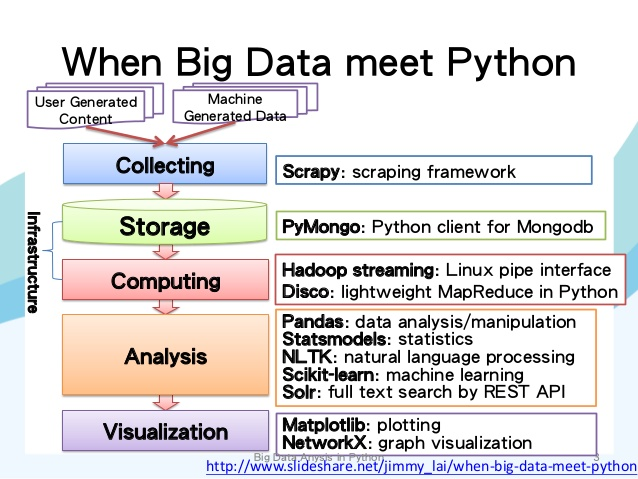
\includegraphics[width=0.99\linewidth]{flowchart}

\end{figure}

\end{frame}
%===========================================================%
\begin{frame}
	\frametitle{Continuum Analytics’ Anaconda}
	\begin{figure}
\centering
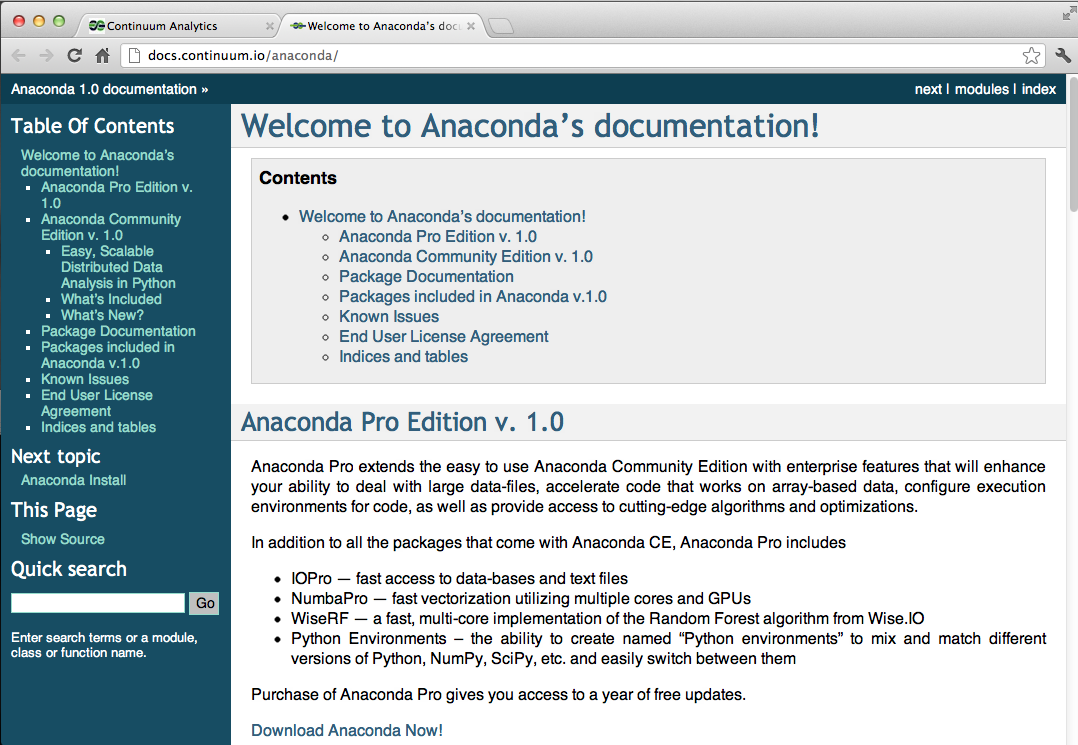
\includegraphics[width=1.0\linewidth]{anaconda.png}

\end{figure}

\end{frame}
%===========================================================%
\begin{frame}
\frametitle{Continuum Analytics’ Anaconda}
\Large
\textbf{Anaconda}
\begin{itemize}
\item Anaconda, a free product of Continuum Analytics (\textit{www.continuum.io}), is a virtually complete scientific
stack (i.e. distribution) for Python. 
\item It includes both the core Python interpreter and standard libraries as well as most
modules required for data analysis. 

\end{itemize}
\end{frame}
%===========================================================%
\begin{frame}
\frametitle{Continuum Analytics’ Anaconda}
\Large
\textbf{Anaconda}
	\begin{itemize}
\item Anaconda is free to use and modules for accelerating the performance
of linear algebra on Intel processors using the \textbf{Math Kernel Library} (MKL) are available (free to
academic users and for a small cost to non-academic users). 
\item Continuum Analytics also provides other
high-performance modules for reading large data files or using the GPU to further accelerate performance
for an additional, modest charge. 
	\end{itemize}

\end{frame}
%===========================================================%
%\begin{frame}[fragile]
%\frametitle{Installing Anaconda}
%\Large
%Most importantly, installation is extraordinarily easy onWindows, Linux
%and OS X. Anaconda is also simple to update to the latest version using
%\begin{framed}
%\begin{verbatim}
%conda update conda
%conda update anaconda
%\end{verbatim}
%\end{framed}
%\end{frame}


\begin{frame}
	\begin{figure}
\centering
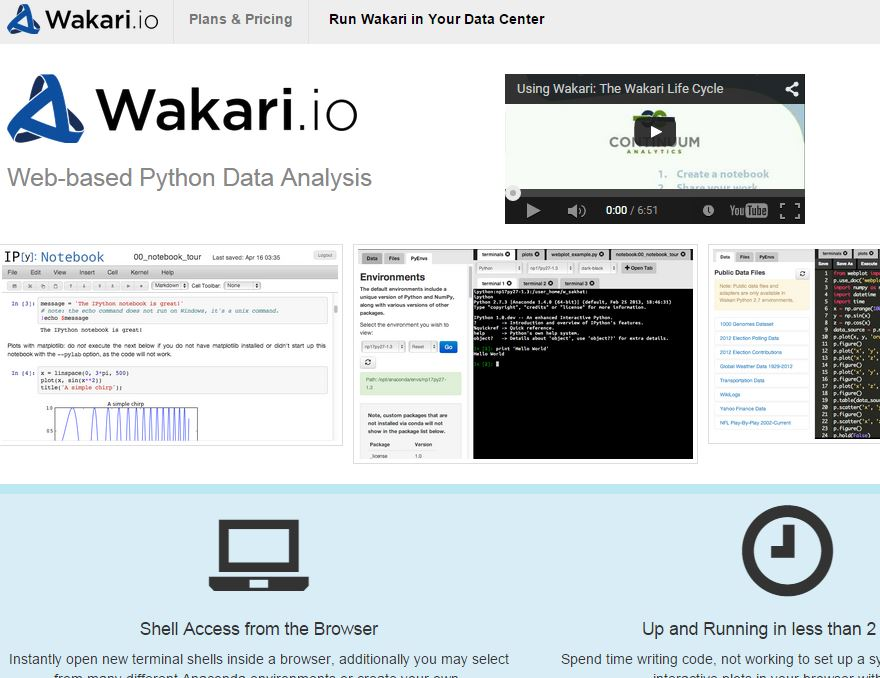
\includegraphics[width=1.1\linewidth]{wakarisite}

\end{figure}

\end{frame}
\begin{frame}
\Large
\textbf{Wakari}\\
\textit{
Wakari is a collaborative data analytics platform that includes tools to explore data, develop analytics scripts, collaborate with IPython notebooks, visualize, and share data analysis and findings. Save time and money by getting right down to business analyzing data with the fully-configured Wakari. In the cloud or on your own servers, Wakari makes accessing your compute resources and data, reproducing your process, and sharing your results easy.}\\(\textbf{Source: Continuum Analytics})
\end{frame}

	
%%===========================================================%
%\textit{\begin{frame}
%\frametitle{NumPy and SciPy}
%
%\begin{itemize}
%\item \textbf{NumPy} provides a set of array and matrix data types which are essential for statistics and econometrics.
%
%\item \textbf{SciPy} contains a large number of routines needed for analysis of data.The most important include a wide
%range of random number generators, linear algebra routines and optimizers. 
%
%\item Remark: SciPy depends on NumPy.
%
%\item More on them later.
%\end{itemize}
%\end{frame}}
%===========================================================%
\begin{frame}
\frametitle{IPython and IPython Notebooks}
\textbf{IPython}
\begin{itemize}
\item IPython provides an interactive Python environment which enhances productivity when developing code
or performing interactive data analysis.
\item

The IPython Notebook is a web-based interactive computational environment where you can combine code execution, text, mathematics, plots and rich media into a single document.

\end{itemize}
\Large
\end{frame}
%===========================================================%
\begin{frame}
\textbf{IPython Notebook}
	\begin{figure}
\centering
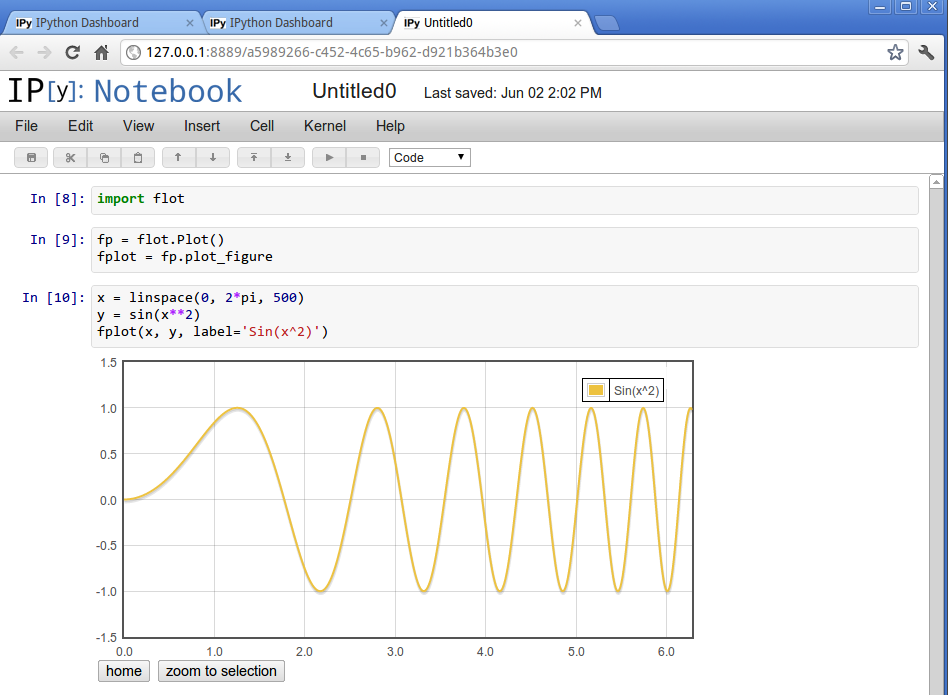
\includegraphics[width=0.99\linewidth]{vk2Q6}

\end{figure}

\end{frame}
%===========================================================%

\begin{frame}
	\textbf{Ipython Notebook / Jupyter}
	\vspace{-0.4cm}
	\begin{figure}
\centering

\includegraphics[width=0.8\linewidth]{jupyter}

\end{figure}

\end{frame}
	
\begin{frame}
	\begin{figure}
\centering
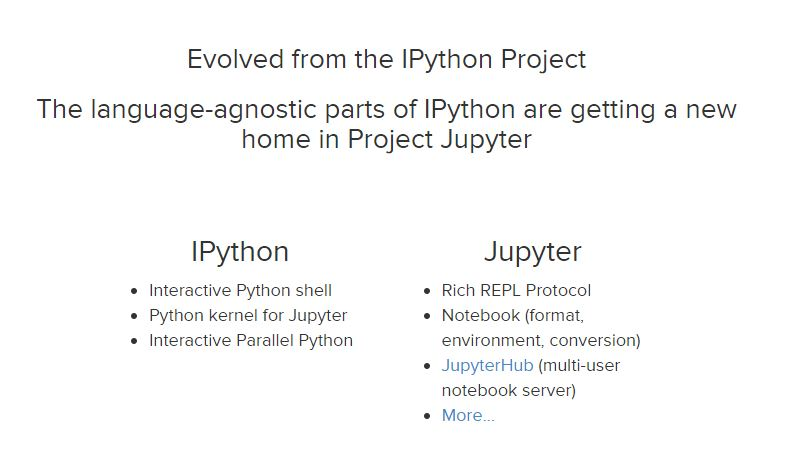
\includegraphics[width=1.0\linewidth]{jupytersiteinfo}

\end{figure}

\end{frame}
\begin{frame}
	\textbf{Markdown}
	\\
	Markdown is a text-to-HTML conversion tool for web writers. Markdown allows you to write using an easy-to-read, easy-to-write plain text format, then convert it to structurally valid XHTML (or HTML).
	\begin{figure}
\centering
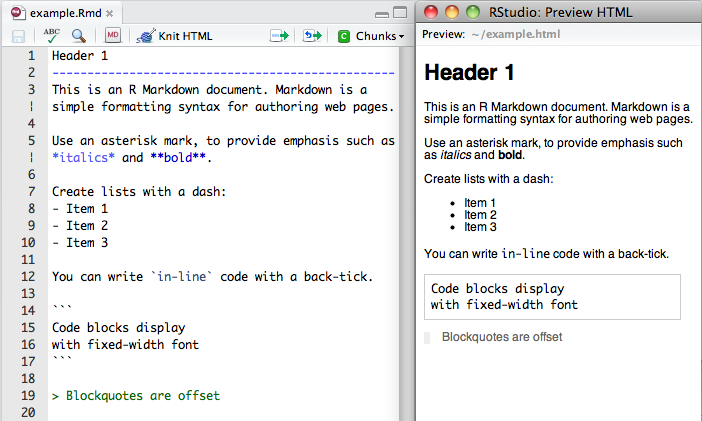
\includegraphics[width=0.80\linewidth]{markdownOverview}

\end{figure}

\end{frame}

%=======================================================================%
\end{document}